% =====================================================================
%  c24 —— 原文印刷页 192--199（PDF 第 193--200 页）
%  含：附录 E 的 E.6（拉格朗日分解的群论解释）、E.7（Hermitian 全纯线丛）及其
%      E.7.1、E.7.2；E.8、E.9（原稿仅存标题与占位说明）；附录 F（Hodge 理论与
%      解析挠率，含 F.1、F.2）；附录 G 的节标题与 G.1（结构群约化：一般讨论）
%  编号公式：(E.46)--(E.68)、(F.1)--(F.21)、(G.1)、(G.2)，共 46 条
%  插图：Fig. 33（印刷第 196 页）、Fig. 34（印刷第 197 页）
%  全部公式逐条对照 150 dpi 页面图像转写。
%  注意：work/chunks/c24.txt 的内容实为印刷页 200--210（即 c25 的正文），
%        与本片段页码范围不符；本片段一律以页面图像为准。
% =====================================================================

\subsection{拉格朗日分解：群论解释} % 原文: E.6 Lagrangian Decomposition: Group-Theoretic Interpretation

回到 Heisenberg 群 $\tilde V$：理解 $\tilde V$ 的一种方式是把它看成由形如
$U(v) := \exp[i(q^I\hat\alpha_I + p_I\hat\beta^I)]$ 的算符构成的群，其中
\begin{equation}
  [\hat\alpha_I, \hat\beta^J] = -2\pi i\,\delta_I{}^J
  \tag{E.46}
  \label{eq:E.46}
\end{equation}

% [Tutor Note: (E.46) 的 $-2\pi i$ 是作者的约定，取这个值才能使 $U(v)U(w)$ 的
% 相位恰为 $e^{i\pi\Omega(v,w)}$——也就是 (E.48)、(E.49) 中出现的那种「$\pi$ 而不是
% $2\pi$」的相位。若按教科书的 $[\hat q,\hat p]=i\hbar$ 直接搬用（等价于把系数取成
% $-i$ 而非 $-2\pi i$），群律就会差一个 $2\pi$，与 (E.47)--(E.49) 里 $H$ 的归一化
% 不再匹配。]

{\small\itshape ［原文标记：需要补充关于 Heisenberg 群的 SvN（Stone--von Neumann）表示之间关系的内容。］}
% [原文待办标记，原文 p.192：**** NEED TO ADD SOMETHING ABOUT THE RELATION TO SvN REPRESENTATIONS OF THE HEISENBERG GROUP ****]

\subsection{Hermitian 全纯线丛} % 原文: E.7 Hermitian Holomorphic Line Bundles

我们希望定义一个与上述 Heisenberg 群同构的复解析群（其中我们用 $\mathbb{C}^*$ 作中心扩张）。为此我们引入：
\begin{equation}
  H(v^+,w^+) := \Omega(Jv,w) + i\Omega(v,w) = g(v,w) + i\Omega(v,w)
  \tag{E.47}
  \label{eq:E.47}
\end{equation}

% [Tutor Note: (E.47) 的记号是混用的：左端把 $H$ 的自变量写成 $v^+,w^+\in V^+$，
% 右端却用实向量 $v,w\in V$（即 $v^+$ 的实部）。同时 $\Omega(Jv,w)=g(v,w)$ 这一
% 等式说明了 $J$ 与度量 $g$ 的相容性，验证 (E.49) 时必须靠它把分母中的
% $\Omega(Jv,v),\Omega(Jw,w)$ 与分子中的 $\Omega(J(v+w),v+w)$ 配对展开。]

注意 $H(iv^+,w^+) = iH(v^+,w^+)$ 而 $H(v^+,iw^+) = -iH(v^+,w^+)$，故 $H$ 是一个
Hermitian 型。由于 $H$ 是 $v^+,w^+$ 的全纯函数，我们可以用 $\mathbb{C}^*$ 作全纯延拓：
\begin{equation}
  (v^+,z)(w^+,z') = \left(v^+ + w^+,\ zz'\,e^{\pi H(v^+,w^+)}\right)
  \tag{E.48}
  \label{eq:E.48}
\end{equation}
这就定义了一个群 $\tilde V^+$。注意上链 $e^{i\pi\Omega(v,w)}$ 与 $e^{\pi H(v^+,w^+)}$
相差一个上边界（coboundary），因为
\begin{equation}
  e^{\pi g(v,w)} = e^{\pi\Omega(Jv,w)}
  = \frac{e^{\frac{\pi}{2}\Omega(J(v+w),v+w)}}
         {e^{\frac{\pi}{2}\Omega(Jv,v)}\,e^{\frac{\pi}{2}\Omega(Jw,w)}}
  = \frac{e^{\frac{\pi}{2}g(v+w,v+w)}}
         {e^{\frac{\pi}{2}g(v,v)}\,e^{\frac{\pi}{2}g(w,w)}}
  \tag{E.49}
  \label{eq:E.49}
\end{equation}
因此 (E.48) 作为群与我们先前的 $\mathbb{C}^*$ 扩张同构。

现在，要在 $V/\Lambda = V^+/\Lambda^+$ 上定义全纯 $\mathbb{C}^*$ 丛，与以前一样我们必须选取一个分裂（splitting），现在它由满足下式的映射 $\lambda\to\tilde\epsilon_\lambda$ 给出：
\begin{equation}
  \tilde\epsilon_\lambda\tilde\epsilon_\mu
  = \tilde\epsilon_{\lambda+\mu}\,e^{-\pi H(\lambda^+,\mu^+)}
  \tag{E.50}
  \label{eq:E.50}
\end{equation}
于是该 $\mathbb{C}^*$ 丛可以描述为群商 $\tilde V^+/\Lambda_{\tilde\epsilon}$
\begin{equation}
  (v^+,z)\sim(v^+,z)(\lambda^+,\tilde\epsilon_\lambda)
  = \left(v^+ + \lambda^+,\ \tilde\epsilon_\lambda\,e^{\pi H(v^+,\lambda^+)}\cdot z\right)
  \tag{E.51}
  \label{eq:E.51}
\end{equation}
若 $z\in\mathbb{C}^*$，我们得到复环面上的一个全纯主 $\mathbb{C}^*$ 丛；若 $z\in\mathbb{C}$，则得到与之相伴的全纯主丛，也就是全纯线丛。

用我们先前讨论的说法，乘子系统（multiplier system）由下式定义
\begin{equation}
  e_\lambda(v^+) = \tilde\epsilon_\lambda\,e^{\pi H(v^+,\lambda^+)}
  \tag{E.52}
  \label{eq:E.52}
\end{equation}

% [Tutor Note: (E.50) 与 (E.51) 的相位符号相反（一个 $e^{-\pi H}$、一个
% $e^{+\pi H}$），这不是笔误：正是这一对相反符号保证 (E.51) 定义的等价关系满足
% 结合律，也保证截面条件 (E.53) 的相容性。核对办法是练习 a.) 的 cocycle 约束
% 与 (E.54) 的换算；若两处同号，(E.53) 将变成反号的拟周期性。]

截面可以提升为 $V^+$ 上的整函数，满足
\begin{equation}
  \vartheta(v^+ + \lambda^+) = e_\lambda(v^+)\,\vartheta(v^+)
  \tag{E.53}
  \label{eq:E.53}
\end{equation}

{\small\itshape ［原文标记：此处需要不变范数——要在该全纯线丛上取得一个 Hermitian 度量。］}
% [原文待办标记，原文 p.193：**** INVARIANT NORM HERE: GET HERMITIAN METRIC ON THE HOLOMORPHIC LINE BUNDLE ****]

若 $d_1 = d_2 = \cdots = d_n = 1$，这样的函数在相差一个常数的意义下应当是唯一的。下一节我们将把它构造出来。

\paragraph{练习}
\begin{enumerate}[label=(\alph*)]
  \item 显式验证 $e_\lambda(v^+)$ 满足上链（cocycle）约束。
  \item 证明：给定 $\epsilon_\lambda$，我们可以按如下方式构造 $\tilde\epsilon_\lambda$：
\begin{equation}
  \tilde\epsilon_\lambda
  = \epsilon_\lambda\,e^{\frac{\pi}{2}\Omega(J\lambda,\lambda)}
  = \epsilon_\lambda\,e^{\frac{\pi}{2}H(\lambda^+,\lambda^+)}
  = \epsilon_\lambda\,e^{\frac{\pi}{2}g(\lambda,\lambda)}
  \tag{E.54}
  \label{eq:E.54}
\end{equation}
\end{enumerate}

\paragraph{练习}
说明如何引入一个简单的前因子（prefactor），从而用经典 theta 函数解出方程 \eqref{eq:E.53}。

首先，利用拉格朗日分裂我们看到可以把 $\epsilon_\lambda$ 写成如下形式：
\begin{equation}
  \epsilon_\lambda = e^{i\pi\lambda_2\lambda^1 + 2\pi i(\theta\cdot\lambda_2 - \phi\cdot\lambda^1)}
  \tag{E.55}
  \label{eq:E.55}
\end{equation}
其中 $\theta,\phi$ 为某两个量。

现在在 $V^+$ 上定义
\begin{equation}
  B(v,w) = v^{tr}Y^{-1}w
  \tag{E.56}
  \label{eq:E.56}
\end{equation}
并计算
\begin{equation}
  (H - B)(v,w) = -2i\,v w^1
  \tag{E.57}
  \label{eq:E.57}
\end{equation}
也就是说，
\begin{equation}
  H(v,w) = v^{tr}Y^{-1}\bar w
  \tag{E.58}
  \label{eq:E.58}
\end{equation}

% [Tutor Note: (E.57) 原文写成 $(H-B)(v,w) = -2ivw^1$，右端只标出了一个指标
% （$w$ 的第 1 个分量），另一个因子按 (E.58) 应理解为与之配对的 $v$ 分量。这一项
% 正是 $H$ 与 $B$ 只差 $\bar w$ 与 $w$ 的体现：按 (E.56)、(E.58)，凡 $Y^{-1}$ 作用到
% 的分量不含第 1 个方向时，$H$ 与 $B$ 的两项完全相同而相消，剩下的只有含 $w^1$
% 的那一部分。照抄时不要把 $v w^1$ 误当成标量乘积 $v\cdot w$。]

于是
\begin{equation}
  \tilde\epsilon_\lambda\,e^{\pi H(v^+,\lambda^+)}
  \frac{e^{\frac{\pi}{2}B(v^+,v^+)}}
       {e^{\frac{\pi}{2}B(v^+ + \lambda^+,v^+ + \lambda^+)}}
  \tag{E.59}
  \label{eq:E.59}
\end{equation}
由下式给出
\begin{equation}
  e^{-i\pi\lambda^1\tau\lambda^1 - 2\pi i v\lambda^1 + 2\pi i(\theta\lambda_2 - \phi\lambda^1)}
  \tag{E.60}
  \label{eq:E.60}
\end{equation}
证明这正是经典 theta 函数的自守因子（factor of automorphy）。

因此，方程 \eqref{eq:E.53} 的 theta 函数与经典 theta 函数通过 $\exp[\frac{\pi}{2}B(v^+,v^+)]$ 相联系。

\subsubsection{计算第一 Chern 类} % 原文: E.7.1 Computing The First Chern Class

当 $L$ 是全纯丛时还有另一种观点：若 $s$ 是 $L$ 的一个整体定义的全纯截面，它将在某个全纯超曲面 $D$ 上为零。于是 $D$ 的 Poincaré 对偶将表示 $c_1(L)$。为得到显式的微分形式，可以在 $L$ 上取一个 Hermitian 度量 $h$：这样 $\|s\|^2 = h(z,\bar z)|s(z)|^2$ 就是 $M$ 上整体良定义的 $C^\infty$ 函数。于是
\begin{equation}
  \frac{1}{2\pi i}\partial\bar\partial\log\|s\|^2
  \tag{E.61}
  \label{eq:E.61}
\end{equation}
是一个闭的 $(1,1)$ 形式，它表示 $c_1(L)$。

为看清这一点，在 $D$ 上某点的附近我们可以取全纯坐标 $(z_1,\dots,z_n)$，使 $D$ 由简单方程 $z_1 = 0$ 定义。

现在回忆，在一个复维的情形：
\begin{equation}
  \nabla^2\log|z|^2 = 4\pi\delta^2(z)
  \tag{E.62}
  \label{eq:E.62}
\end{equation}
或者换个说法，若 $\partial_z = \frac{1}{2}(\partial_x - i\partial_y)$，则
\begin{equation}
  \partial_z\partial_{\bar z}\log|z|^2 = \pi\delta^2(z)
  \tag{E.63}
  \label{eq:E.63}
\end{equation}
因此，在这些局部坐标下
\begin{equation}
  \frac{1}{2\pi i}\partial\bar\partial\log\|s\|^2
  = \delta^2(z)\,\frac{dz_1\wedge d\bar z_1}{2i}
  \tag{E.64}
  \label{eq:E.64}
\end{equation}

% [Tutor Note: 从 (E.62) 到 (E.63) 只用了 $\partial_z\partial_{\bar z}=\frac14\nabla^2$，
% 因子 $4$ 与 $\pi$ 的对应关系全在这一步；另外 $\delta^2(z)$ 指二维 delta
% $\delta(x)\delta(y)$，不是 $\delta(z)$（后者不是分布）。核对 (E.64) 时还应注意
% 右边是 $(1,1)$ 形式 $\frac{dz_1\wedge d\bar z_1}{2i}$，其系数与 $\delta^2$ 的
% 归一化必须一起看，否则 $c_1$ 的整性（对 $D$ 的积分）会差一个因子。]

然而注意，上式的左端是整体良定义的。我们已在坐标中局部地取 $h(z,\bar z) = 1$。若它不同，我们只会把 $c_1(L)$ 的代表元改变一个恰当形式。

\subsubsection{全纯截面的一组基：第 $\kappa$ 级 theta 函数} % 原文: E.7.2 A Basis Of Holomorphic Sections: Level κ Theta Functions

我们定义第 $\kappa$ 级 theta 函数为
\begin{equation}
  \Theta_{\beta,\kappa}(\xi,\tau)
  = \sum_{s_I\in\mathbb{Z}}
    e^{2\pi i\kappa\left(s_I+\frac{1}{2\kappa}\beta_I\right)\tau^{IJ}
          \left(s_I+\frac{1}{2\kappa}\beta_I\right)}
    e^{2\pi i\xi^I(2\kappa s_I+\beta_I)}
  \tag{E.65}
  \label{eq:E.65}
\end{equation}
% [原文如此：(E.65) 指数里两处括号的下标都写作 $s_I$（而不是 $s_J$），与 $\tau^{IJ}$
%  的一对上指标不匹配；按原文逐字转写，未作改动。正确的求和约定应是
%  $s_I\,\tau^{IJ}s_J$，即 $I$ 与 $J$ 各出现两次。]
（它们与前面讨论的 Riemann theta 函数只是简单相关。）

$I = 1,\dots,g$。

$\Theta_{\beta,\kappa}$ 只依赖于 $\beta$ 到 $\mathbb{Z}^g/(2\kappa\mathbb{Z})^g$ 的投影。$\xi$ 的线性无关函数共有 $(2\kappa)^g$ 个。

{\small\itshape ［原文标记（页边注）：不要用 $\tau^{IJ}$！！那看起来像 $\tau$ 的逆。需要把这些方程改回 $\tau_{IJ}$。］}
% [原文待办标记，原文 p.194 右侧页边注：\ensuremath{\clubsuit} Don't use τ^{IJ} !! That looks like the inverse of τ. Need to convert these equations back to τ_{IJ}. \ensuremath{\clubsuit}]
% [Tutor Note: 按作者的这条页边注，(E.65)、(E.66)、(E.68) 中的 $\tau^{IJ}$
% 应当读作周期矩阵本身 $\tau_{IJ}$（不取逆）；作者只是把指标写成上标，与真正的
% 逆矩阵记号冲突。若照字面把它当逆矩阵，则 (E.66) 第二行的相位与 $\Theta$ 的
% 拟周期性不再自洽。]

$T = V_{\mathbb{R}}/V_{\mathbb{Z}}$ 是主极化（principally polarized）簇（也就是说，辛形式的不变量 $d_i = 1$）。此外，如我们已经看到的，$\Theta_{\beta,\kappa}(\xi,\tau)$ 是线丛 $\mathcal{L} = L^{\otimes 2\kappa}\to T$ 的一个截面。若 $\mu$ 是整向量：
\begin{equation}
\begin{aligned}
  \Theta_{\beta,\kappa}(\xi+\mu,\tau) &= \Theta_{\beta,\kappa}(\xi,\tau)\\
  \Theta_{\beta,\kappa}(\xi+\tau\mu,\tau)
  &= e^{-2\pi i\kappa\mu_I\tau^{IJ}\mu_J - 4\pi i\kappa\xi^I\mu_I}
     \,\Theta_{\beta,\kappa}(\xi,\tau)
\end{aligned}
\tag{E.66}
\label{eq:E.66}
\end{equation}
因此，
\begin{equation}
  \|\Theta_{\beta,\kappa}(\xi,\tau)\|^2
  := e^{-4\pi\kappa(\operatorname{Im}\xi^I)Y_{IJ}^{-1}(\operatorname{Im}\xi^J)}
     \,\Theta_{\beta,\kappa}(\xi,\tau)\overline{\Theta_{\beta',\kappa}(\xi,\tau)}
  \tag{E.67}
  \label{eq:E.67}
\end{equation}
是不变的——它是环面上光滑定义的函数。现在我们来计算 $c_1(\mathcal{L})$ 的代表元：
\begin{equation}
  \omega = \frac{1}{2\pi i}\partial\bar\partial\log\|s\|^2 = 2\kappa\,dx^I dy_I
  \tag{E.68}
  \label{eq:E.68}
\end{equation}
其中 $\xi^I = x^I + \tau^{IJ}y_J$，$x^I,y^I$ 为实。

对 $\kappa = \frac{1}{2}$，我们得到环面上体积为 $1$ 的基本辛形式。

{\small\itshape ［原文标记：此处原稿留有一对星号括起的空行，占位内容未写出。］}
% [原文待办标记，原文 p.195：一对 **** 之间为空，作者尚未填入内容]

\subsection{模变换律} % 原文: E.8 Modular Transformation Laws

{\small\itshape ［本节在原稿中仅有标题，正文尚未写出。］}
% [原文状况说明，原文 p.195：E.8 标题之下直接接 E.9 标题，无任何正文。相关内容
%  在 E.7 末以经典 theta 函数自守因子的形式出现（见 (E.55)--(E.60) 及随后练习）。]

\subsection{热方程} % 原文: E.9 The Heat Equation

{\small\itshape ［原文标记：热方程——更多材料见 Freed--Moore--Segal, 2006, [20], 第 6 节。］}
% [原文待办标记，原文 p.195：HEAT EQUATION / MORE MATERIAL IN: Freed-Moore-Segal, 2006, [20], section 6.]

\section{Hodge 理论与解析挠率} % 原文: F. Hodge Theory And Analytic Torsion

\begin{keytakeaways}
  \item 定义：解析挠率（analytic torsion，又称 Ray--Singer 挠率）由
    $\tau=\int_0^\infty\frac{dt}{t}\operatorname{Tr}F(-1)^Fe^{-tH}$ 给出，迹取在 de Rham 复形上；
    它用度规的 Laplacian 行列式表达，却是闭流形的拓扑不变量。
  \item 星算符代数：$*^2=(-1)^{k(n-k)}$，故 $n$ 偶时 $*^2=(-1)^F$、$n$ 奇时 $*^2=+1$；
    由此 $d^\dagger=(-1)^{nF+1}*d*$，正定 Hamilton 量在两种维数下形式不同（$n$ 奇时多一个 $(-1)^F$），见 (F.5)--(F.9)。
  \item 度规无关性的机制：$\dot\tau$ 化成 $-\frac{d}{dt}\operatorname{Tr}(-1)^Fue^{-tH}$ 的积分；
    上端由 $e^{-tH}$ 的衰减给出零，下端由 $*$ 在偶/奇子复形上均为等距、使 $\operatorname{Tr}(-1)^Fu$ 形式为零给出零。
  \item 三维流形的结果：$\tau=-\log\det\Delta^{(1)}+2\log\det\Delta^{(2)}-3\log\det\Delta^{(3)}$，
    谱乘积形式表明 $\Omega^1,\Omega^2$ 的贡献只经由 $(\mu_n^{(1)})^2$ 与 $(\lambda_n^{(0)})^2$ 进入。
  \item 图像：图 33 给出 $T$ 在 $(\ker T)^\perp$ 与 $(\ker T^\dagger)^\perp$ 之间的同构；
    图 34 把这套正交分解画到三维流形的 de Rham 复形上，$*$ 是关于中心竖直线的等距翻转。
\end{keytakeaways}

解析挠率（analytic torsion），又称 Ray--Singer 挠率，是 $n$ 维闭流形 $M$ 的一个拓扑不变量。但它要用微分形式上的 Laplacian 的行列式来表达。

\subsection{一些 Hodge 理论} % 原文: F.1 Some Hodge Theory

在任何流形上我们都有 de Rham 复形：$d:\Omega^*(M)\to\Omega^*(M)$。我们把微分形式的次数 $k$ 称为「费米子数」，因为它与一个在 $M$ 上运动的粒子的超对称量子力学有关。于是费米子数算符 $F$ 就是作用在 $\Omega^k(M)$ 上的 $F = k$。

若给 $M$ 一个 Riemann 度量，我们就可以谈论 $L^2$ 形式。它们构成该超对称量子力学的 Hilbert 空间。

若 $M$ 此外还有 Riemann 度量，我们可以定义 Hodge 星算符：
\begin{equation}
  *:\Omega^k(M)\to\Omega^{n-k}(M)
  \tag{F.1}
  \label{eq:F.1}
\end{equation}

作用在 $\Omega^k(M)$ 上的 Hodge 对偶满足
\begin{equation}
  \alpha\wedge*\beta
  = \frac{1}{k!}\,g^{\mu_1\nu_1}\cdots g^{\mu_k\nu_k}
    \alpha_{\mu_1\cdots\mu_k}\beta_{\nu_1\cdots\nu_k}\operatorname{vol}(g)
  \tag{F.2}
  \label{eq:F.2}
\end{equation}
而这个方程已足以定义它。

记住下面这一点是有用的：若 $\omega_1\in\Omega^k(M_{n_1})$、$\omega_2\in\Omega^j(M_{n_2})$ 且
$g = g_1\oplus g_2$，并给乘积流形 $M_1\times M_2$ 以定向
$\operatorname{vol}(g_1)\wedge\operatorname{vol}(g_2)$，则
\begin{equation}
  *(\omega_1\wedge\omega_2)
  = (-1)^{j(n_1-k)}(*_1\omega_1)\wedge(*_2\omega_2)
  \tag{F.3}
  \label{eq:F.3}
\end{equation}

还注意到
\begin{equation}
  *^2 = \operatorname{sign}(\det g)(-1)^{k(n-k)}
  \tag{F.4}
  \label{eq:F.4}
\end{equation}
作用在 $k$ 形式上。这里我们将只考虑 Riemann 度量，它们是正定的。因此
\begin{equation}
  *^2 = (-1)^{k(n-k)} = (-1)^F(-1)^{nF} = (-1)^{(n+1)F}
  = \begin{cases}
      (-1)^F & n = 0\ (2)\\
      +1 & n = 1\ (2)
    \end{cases}
  \tag{F.5}
  \label{eq:F.5}
\end{equation}

% [Tutor Note: (F.5) 中间两个等号各跳过一步。其一，$F$ 在 $\Omega^k$ 上取 $k$，
% 故 $(-1)^F(-1)^{nF}=(-1)^{(n+1)F}$ 是逐特征子空间成立；其二，
% $(-1)^{k(n-k)}=(-1)^{kn-k^2}=(-1)^{kn-k}$（因为 $k^2\equiv k \bmod 2$），
% 而 $(-1)^{(n+1)k}=(-1)^{nk+k}$，两者相差 $(-1)^{2k}=1$。最后一步：$n$ 偶时
% $(-1)^{(n+1)F}=(-1)^F$，$n$ 奇时 $(-1)^{(n+1)F}=+1$。若把 $F$ 当成普通整数
% $k$ 直接代入，容易漏掉 $k^2\equiv k$ 这一同余。]

对单参数度规族 $g(s)$，其导数满足
\begin{equation}
  \dot{*}* + *\dot{*} = 0
  \tag{F.6}
  \label{eq:F.6}
\end{equation}
于是
\begin{equation}
  u = \dot{*}*^{-1} = -*^{-1}\dot{*}
  \tag{F.7}
  \label{eq:F.7}
\end{equation}

又有
\begin{equation}
  d^\dagger = (-1)^{nF+1}*d* = (-1)^{nF+1}\delta
  \tag{F.8}
  \label{eq:F.8}
\end{equation}

正定的 Hamilton 量
\begin{equation}
  H = dd^\dagger + d^\dagger d
  = (-1)^{nF+1}\left(\delta d + (-1)^n d\delta\right)
  = \begin{cases}
      -(*d*d + d*d*) & n = 0\ (2)\\
      -(-1)^F(*d*d - d*d*) & n = 1\ (2)
    \end{cases}
  \tag{F.9}
  \label{eq:F.9}
\end{equation}

% [Tutor Note: 这里的 $F$ 出现在指数里时是算符（在 $\Omega^k$ 上取 $k$），
% 所以 $(-1)^{nF+1}$ 是分次符号，不能当成常数。与常见教科书写法
% $d^\dagger=(-1)^{nk+n+1}*d*$ 对照即可核对：在 $k$ 形式上 $nF=nk$。
% 代入 (F.9) 第一种情形（$n$ 偶）时 $(-1)^{nF+1}=-1$，故整体变号；第二种情形
% 还要额外提出 $(-1)^F$，这是 $\delta d$ 与 $d\delta$ 在 $n$ 奇时相对符号的来源。]

\begin{figure}[htbp]
  \centering
  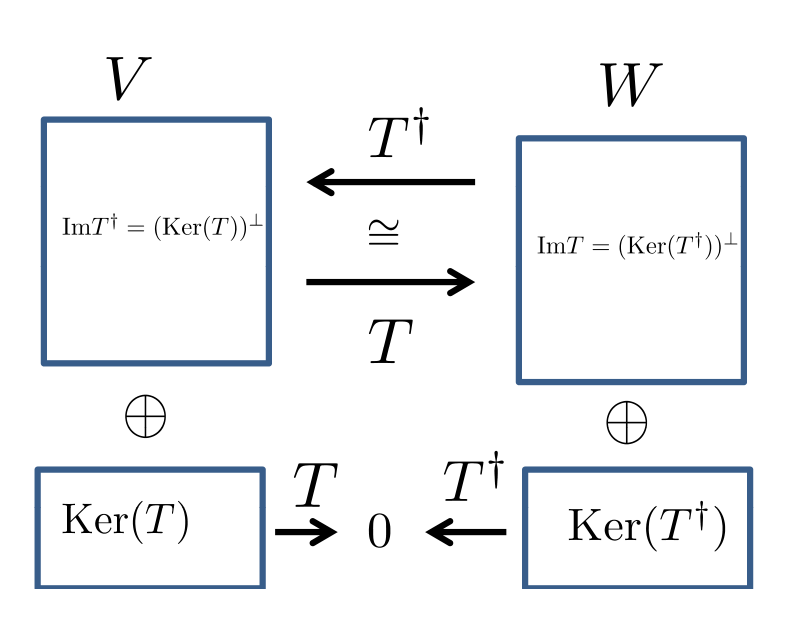
\includegraphics[width=0.72\textwidth]{figures/fig33.png}
  \caption{内积空间之间算符 $T$ 的定义域与值域的正交分解。（原文 Fig.~33，第 196 页）}
  \label{fig:33}
\end{figure}

若 $V,W$ 是内积空间，而 $T:V\to W$ 是一个（足够好的）线性算符，则 $T$ 限制为
$(\ker T)^\perp$ 与 $(\ker T^\dagger)^\perp$ 之间的一个同构，如 33 所示。把它应用于三维的 de Rham 复形，我们便得到这样一幅图景：

{\small\itshape ［原文标记：把 $*$ 解释为等距同构，以及三维流形的特殊情形：］}
% [原文待办标记，原文 p.196：EXPLAIN * AS ISOMETRY AND SPECIAL CASE OF 3-MANIFOLDS:]

\begin{enumerate}
  \item $d$ 与 $d^\dagger$ 作为超对称算符。
  \item $d^\dagger d$ 在 $\Omega^0$ 上的非零谱就是 $dd^\dagger$ 在 $\Omega^3$ 上的谱。记之为 $(\lambda_n^{(0)})^2$。
  \item 在 $\Omega^1$ 上我们有 $dd^\dagger$，其谱为 $(\lambda_n^{(0)})^2$；我们把 $*d$ 对角化，
    本征值为 $\mu_n^{(1)}$，于是 $d^\dagger d$ 的谱为 $(\mu_n^{(1)})^2$。
  \item 在 $\Omega^2$ 上我们有 $dd^\dagger$，其谱为 $(\mu_n^{(1)})^2$；而 $d^\dagger d$ 的谱为 $(\lambda_n^{(0)})^2$。
\end{enumerate}

\begin{figure}[htbp]
  \centering
  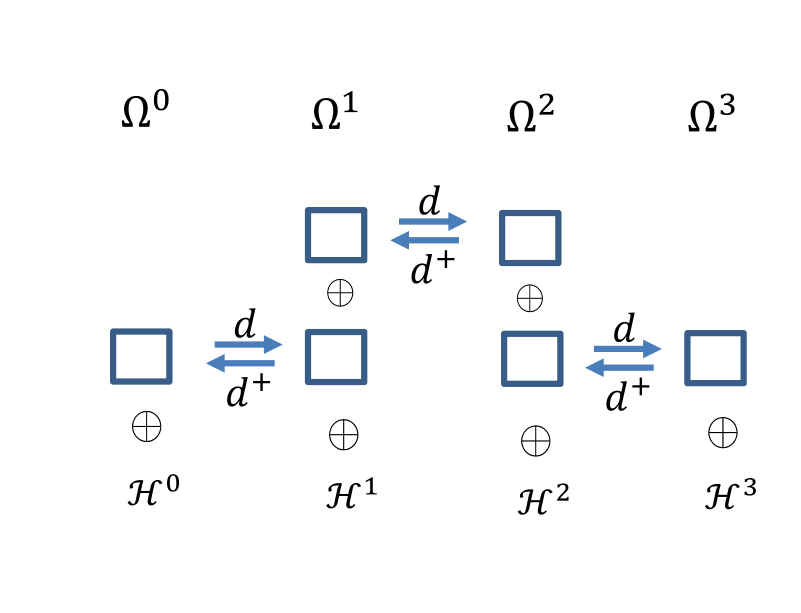
\includegraphics[width=0.80\textwidth]{figures/fig34.png}
  \caption{Riemann 三维流形上 de Rham 复形的 Hodge 分解图示。水平箭头是 Hilbert 空间之间的同构。
    Hodge $*$ 算符是一个等距，它把整幅图关于中心的竖直线翻转过来。这导致解析挠率的有效简化。
    （原文 Fig.~34，第 197 页）}
  \label{fig:34}
\end{figure}

{\small\itshape ［原文标记：图示 Hodge 分解——核对群论笔记。］}
% [原文待办标记，原文 p.197：FIGURE ILLUSTRATING THE HODGE DECOMPOSITION – check Group Theory notes]

\subsection{解析挠率} % 原文: F.2 Analytic Torsion

解析挠率基于如下积分
\begin{equation}
  \tau = \int_0^\infty\frac{dt}{t}\operatorname{Tr}F(-1)^F e^{-tH}
  \tag{F.10}
  \label{eq:F.10}
\end{equation}
其中迹是在 de Rham 复形 $\Omega^*(M)$ 上取的。

基本想法是：若 $\lambda$ 与 $\lambda'$ 有正实部，则
\begin{equation}
  \int_0^\infty\frac{dt}{t}\left(e^{-\lambda t} - e^{-\lambda' t}\right)
  = \log\frac{\lambda'}{\lambda}
  \tag{F.11}
  \label{eq:F.11}
\end{equation}
因此，对两个不同的度规，(F.10) 的两个表达式之差，就是下述量在这两组度规下的差：
\begin{equation}
  \sum_k(-1)^k k\log\operatorname{Det}'(\Delta_k)
  \tag{F.12}
  \label{eq:F.12}
\end{equation}
另一方面，(F.10) 本身是有意义的。我们下面将说明，它与度规无关，因而定义一个拓扑不变量。

这个定义\emph{先验地}依赖于一个度规。取一族度规 $g(s)$ 并对 $s$ 求导：
\begin{equation}
  \dot\tau = -\int_0^\infty dt\,\operatorname{Tr}F(-1)^F\dot H e^{-tH}
  \tag{F.13}
  \label{eq:F.13}
\end{equation}
\begin{equation}
\begin{aligned}
  \dot H &= -(-1)^{nF}\left(\dot{*}d*d + *d\dot{*}d + (-1)^n d\dot{*}d* + (-1)^n d*d\dot{*}\right)\\
  &= -(-1)^{nF}\left(u\delta d - \delta u d + (-1)^n du\delta - (-1)^n d\delta u\right)
\end{aligned}
\tag{F.14}
\label{eq:F.14}
\end{equation}

现在试着把 $-\operatorname{Tr}F(-1)^F\dot H e^{-tH}$ 写成
$\operatorname{Tr}F(-1)^{(n+1)F}ue^{-tH}(\cdots)$ 的形式，必要时循环移动 $d$ 与 $\delta$。注意 $[d,H] = 0$ 且 $[\delta,H] = 0$。

同时我们需要

对 $n = 0\ (2)$：
\begin{equation}
  [F(-1)^F, d] = d(-1)^{F+1}(2F+1)
  \tag{F.15}
  \label{eq:F.15}
\end{equation}
因为 $\left((f+1)(-1)^{f+1} - f(-1)^f\right) = (-1)^{f+1}(2f+1)$。
\begin{equation}
  [F(-1)^F, \delta] = \delta(-1)^{F+1}(2F-1)
  \tag{F.16}
  \label{eq:F.16}
\end{equation}
因为 $\left((f-1)(-1)^{f-1} - f(-1)^f\right) = (-1)^{f-1}(2f-1)$。

对 $n = 1\ (2)$：
\begin{equation}
  [F, d] = d
  \tag{F.17}
  \label{eq:F.17}
\end{equation}
\begin{equation}
  [F, \delta] = -\delta
  \tag{F.18}
  \label{eq:F.18}
\end{equation}

先取 $n = 0\ (2)$。于是我们有
\begin{equation}
\begin{aligned}
  -\operatorname{Tr}F(-1)^F\dot H e^{-tH}
  &= \operatorname{Tr}F(-1)^F\left(u\delta d - \delta u d + du\delta - d\delta u\right)e^{-tH}\\
  &= -\frac{d}{dt}\left(\operatorname{Tr}(-1)^F u e^{-tH}\right)
\end{aligned}
\tag{F.19}
\label{eq:F.19}
\end{equation}

% [Tutor Note: (F.14) 到 (F.19) 之间省略了「循环移动」的全部步骤：把 (F.14) 的
% 四项各自用 $[d,H]=[\delta,H]=0$（故 $e^{-tH}$ 可自由穿过 $d,\delta$）、
% $d^2=\delta^2=0$ 以及 $\operatorname{Tr}$ 的循环性搬到 $u$ 的同侧，再用
% (F.15)--(F.18) 的交换子把 $F$ 的因子提出。搬动过程中穿过 $(-1)^F$ 会带来
% (F.15)--(F.18) 那样的符号；若只把 $d,\delta$ 当普通矩阵交换，会丢掉
% $(-1)^{F+1}(2F\pm1)$ 中的 $2F$ 项，(F.19) 的第二行就不再是全导数。]

现在我们可以分部积分。在 $t = 0$ 附近我们有 $\operatorname{Tr}(-1)^F u e^{-\epsilon H}$。
它是 $\operatorname{Tr}(-1)^F u$ 的一个正则化版本。后者形式上是零，因为 $*$ 同时是 de Rham 复形偶子复形与奇子复形的等距，所以我们是在取一个反对称算符的迹。

现在考虑 $n = 1\ (2)$。
\begin{equation}
\begin{aligned}
  -\operatorname{Tr}F(-1)^F\dot H e^{-tH}
  &= \operatorname{Tr}F\left(u\delta d - \delta u d - du\delta + d\delta u\right)e^{-tH}\\
  &= -\frac{d}{dt}\left(\operatorname{Tr}(-1)^F u e^{-tH}\right)
\end{aligned}
\tag{F.20}
\label{eq:F.20}
\end{equation}

我们再分部积分一次。为处理下限，注意 $u$ 与 $(-1)^F$ 对易，并且也把
$\Omega^k\to\Omega^k$。若它可以对角化，则它在 $\Omega^k$ 与 $\Omega^{n-k}$ 上有相同的本征值，
于是 $(-1)^F u$ 的本征值相反，从而至少在形式上 $\operatorname{Tr}(-1)^F u = 0$。

对三维流形的情形
\begin{equation}
\begin{aligned}
  \tau &= -\log\det\Delta^{(1)} + 2\log\det\Delta^{(2)} - 3\log\det\Delta^{(3)}\\
  &= \log\prod_n(\mu_n^{(1)})^2 - 2\log\prod_n(\lambda_n^{(0)})^2
\end{aligned}
\tag{F.21}
\label{eq:F.21}
\end{equation}

\section{流形上的定向、Spin、Spin$^c$、$Pin^{\pm}$ 与 Pin$^c$ 结构} % 原文: G. Orientation, Spin, Spin^c, Pin^±, And Pin^c Structures On Manifolds

\begin{keytakeaways}
  \item 定义：沿同态 $\phi:G_1\to G_2$ 把主 $G_2$ 丛 $P_2$ 约化到 $G_1$，就是给一个主 $G_1$ 丛 $P_1$
    连同同构 $P_1\times_{G_1}G_2\cong P_2$，即交换图 (G.1)；等价的说法是：过渡函数取在 $G_1$ 中，
    并逐点经 $\phi$ 映到 $G_2$。
  \item 三类几何例子：子群包含（$P/H$ 的截面给出子丛，$H=\{1\}$ 时即「整体截面平凡化丛」）、
    $O(n)\subset GL(n,\mathbb{R})$（Riemann 度量把标架丛约化为正交标架丛）、
    $SO(n)\subset O(n)$（截面即定向）。
  \item 覆盖映射的情形：$\phi:\tilde G\to G$ 满射、核为 $K$ 时，「约化」实际是提升——给的是覆盖 $P$
    的主 $\tilde G$ 丛 $\tilde P$，满足 $\tilde P/K\cong P$（图 (G.2)）；作者本人指出「约化」一词在此有误导。
  \item 本节标题所列的 Spin、Spin$^c$、$Pin^{\pm}$、Pin$^c$ 结构，都将作为上述框架中不同 $\phi$ 的特例出现。
\end{keytakeaways}

\subsection{结构群约化：一般讨论} % 原文: G.1 Reduction Of Structure Group: General Discussion

给定两个紧 Lie 群 $G_1,G_2$ 以及一个同态 $\phi:G_1\to G_2$，我们可以定义一个函子 $F_\phi$，从 $M$ 上的主 $G_1$ 丛到 $M$ 上的主 $G_2$ 丛，其作法是：把主 $G_1$ 丛 $G_1\to P\to M$ 送到 $(P\times_{G_1}G_2)\to M$。回忆 $(P\times_{G_1}G_2)$ 是
对 $(p,g)\in P\times G_2$ 在等价关系 $(ph,g) = (p,\phi(h)g)$（$h\in G_1$）下的等价类之集，且它显然带有一个自由的右 $G_2$ 作用。

\begin{definition}[原文未编号]
  若 $G_2\to P_2\to M$ 是一个主 $G_2$ 丛，则\emph{沿 $\phi:G_1\to G_2$ 到 $G_1$ 的一个约化}
  是一个主 $G_1$ 丛 $G_1\to P_1\to M$ 连同一个同构 $\psi$，使得我们有如下交换图：
\begin{equation}
  \begin{array}{ccc}
    (P_1\times_{G_1}G_2) & \xrightarrow{\ \psi\ } & P_2\\[4pt]
    \searrow & & \downarrow\\[4pt]
    & M &
  \end{array}
  \tag{G.1}
  \label{eq:G.1}
\end{equation}
\end{definition}

把定义展开一遍，就可以用贴片重叠 $\mathcal{U}_{\alpha\beta}$ 上的过渡函数给出描述。若
$h_{\alpha\beta}:\mathcal{U}_{\alpha\beta}\to G_1$ 是 $P_1$ 的过渡函数，则作为主 $G_2$ 丛，$P_2$
与一个过渡函数为 $\phi(h_{\alpha\beta}):\mathcal{U}_{\alpha\beta}\to G_2$ 的丛同构。

\paragraph{例子}
\begin{enumerate}
  \item 若 $\phi:H\to G$ 是一个子群的包含，则给定 $G$ 丛 $P\to M$，$H$ 自由作用，
    于是我们可以考虑 $G/H\to P/H\to M$，即一个齐性空间丛。在此情形，丛 $P/H$ 的一个截面
    给出 $P$ 到 $H$ 丛的一个约化，而后者事实上是一个子丛。作为特例，取 $H = \{1\}$。
    这正是众所周知的事实：主 $G$ 丛的一个整体截面使该丛平凡化。
  \item 取 $H = O(n)$、$G = GL(n,\mathbb{R})$。一个度量把标架丛约化为正交标架丛
    $\mathcal{B}_O(M)$。显然，正交标架丛是标架丛的子丛。
  \item 设 $M$ 是一个 Riemann 流形，$H = SO(n)$、$G = O(n)$，而 $\phi$ 是包含。
    则 $\mathcal{B}_O(M)/H$ 是定向二重覆盖。若 $M$ \emph{可定向}，则定向丛有截面。
    事实上，若 $M$ 连通，$\mathcal{B}_O(M)$ 有两个连通分支，因而有两个截面。
    选取一个截面给出该丛到 $SO(n)$ 定向标架丛的约化。截面的选取就是 $M$ 定向的选取。
  \item 现在设 $\phi$ 是一个覆盖映射，即 $\phi:\tilde G\to G$ 是\emph{满射}、核为 $K$。
    于是把主 $G$ 丛 $P$「约化」为主 $\tilde G$ 丛 $\tilde P$，就是一个同构
\begin{equation}
  \begin{array}{ccc}
    \tilde P/K & \xrightarrow{\ \psi\ } & P\\[4pt]
    \searrow & & \downarrow\\[4pt]
    & M &
  \end{array}
  \tag{G.2}
  \label{eq:G.2}
\end{equation}
\end{enumerate}

% [Tutor Note: 术语取舍。reduction of structure group 译为「结构群约化」，这是中文
% 文献的通行译法；但如第 4 例所示，覆盖映射情形下「约化」得到的 $\tilde P$ 其实是
% $P$ 的提升（覆盖），而不是子丛，作者因此说这个词「有误导性」。另一种译法是
% 「结构群的提升」；本译本统一用「约化」以与原文一致，遇到第 4 例时按此理解即可。]

注意一般定义中的「约化」一词有误导性，因为 $\tilde P$ 实际上是 $P$ 的一个覆盖。换个说法，主 $G$
% [跨页衔接：本句在原文 p.199 底部被截断，后半句「丛 $P$ 到 $\tilde G$ 的约化，等同于
%  一个覆盖 $P$ 的主 $\tilde G$ 丛 $\tilde P$」由下一片段 c25 的开头接续。]
